\documentclass{ctexart}
\def\dd{{\rm d}}
\begin{document}
\title{计算物理作业12}
\author{刘畅, PB09203226}
\maketitle

{\bf [作业12]}: 以 $x_{n+1} = \lambda\sin\pi x_n$ 为迭代方程,
(1) 画出系统状态随参数 $\lambda$ 的变化图; (2)画出相应
的 Lyapunov 指数随参数 $\lambda$ 的变化图.

\section{算法和程序}
为了得到系统在 $n\to\infty$ 时的状态, 我们做足够多次的迭代, 然后输出迭代序列
的接下来一些项. 如果是稳定解的情况, 那么输出的迭代序列基本都是一样的. 如果是
倍周期的情况, 输出的序列在两个值直接振荡. 如果是混沌的情况, 输出在某个区间内
随机振荡. 要实现这个算法, 程序非常简单: (\verb|main.c:print_iter_seq()|)
\begin{verbatim}
#define INIT_X    (0.789)
void print_iter_seq(FILE *fout, double lambda,
                    int nskip, int nsteps)
{
    double x = INIT_X;
    int i;

    /* skip first nskip values in the sequence */
    for (i = 0; i < nskip; i++)
        x = iter_fcn(lambda, x);

    /* print next nsteps values of the iteration sequence */
    for (i = 0; i < nsteps; i++) {
        x = iter_fcn(lambda, x);
        fprintf(fout, "%.12f %.12f\n", lambda, x);
    }
}
\end{verbatim}
上面的代码就是把前面的算法翻译成程序, 首先跳过迭代序列的前面几项, 然后输出
序列的接下来几项. 为了通用起见, 前面的代码中将迭代函数设成了 \verb|iter_fcn()|:
\begin{verbatim}
#define CONST_PI    (4.0*atan(1.0))
double iter_fcn(double lambda, double x)
{
    return lambda * sin(CONST_PI * x);
}
\end{verbatim}

按照定义
\[
\nu = \lim_{n\to\infty}\frac{\ln\frac{\dd x_n}{\dd x_0}}{n}
\]
为了计算 Lyapunov 指数, 只要从 $x_0$ 和 $x_o+\dd x_0$ 开始迭代计算至第 $n$
项即可. 代码如下: (\verb|main.c:get_lyapunov()|)
\begin{verbatim}
double get_lyapunov(double lambda, double x, double delta, int nsteps)
{
    int i;
    double y = x + delta;

    assert(delta > 0);
    for (i = 0; i < nsteps; i++) {
        x = iter_fcn(lambda, x);
        y = iter_fcn(lambda, y);
    }
    return (log(fabs(y-x) / delta)) / nsteps;
}
\end{verbatim}
如果 \verb|log| 的参数过小, 那么函数返回的结果是 \verb|-inf|, 在下面的作图
中不能显示出点来. 其他部分没有什么好解释的, 就是把上面的算法翻译成 C 语言.

为了便于比较, 也由于代码组织的方式使得这样做很容易, 我们可以对 Logistic 映射
$y = \lambda x(1-x)$ 做同样的事情: (\verb|logistic.c:iter_fcn()|)
\begin{verbatim}
double iter_fcn(double lambda, double x)
{
    return lambda * x * (1-x);
}
\end{verbatim}
其余的代码完全一样, 在 \verb|logistic.c|. 前面的代码在 \verb|main.c|.

\section{结果}
用 \verb|gnuplot| 作图(作图代码见 \verb|Makefile|), 对原问题, 状态随 $\lambda$
的图:
\begin{center}
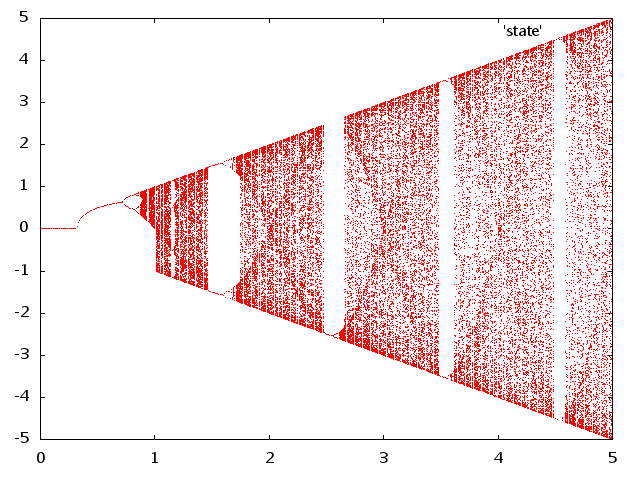
\includegraphics[width=4in]{state.png}
\end{center}
可以看到从一个 $\lambda_0<1$ 开始系统有倍周期分叉的现象.
$\lambda=1$ 开始系统就进入了混沌状态.

然后是 Lyapunov 指数随 $\lambda$ 的关系. 图上空的点对应的指数是 $-\infty$.
可以看到和上面的状态图是一致的.
\begin{center}
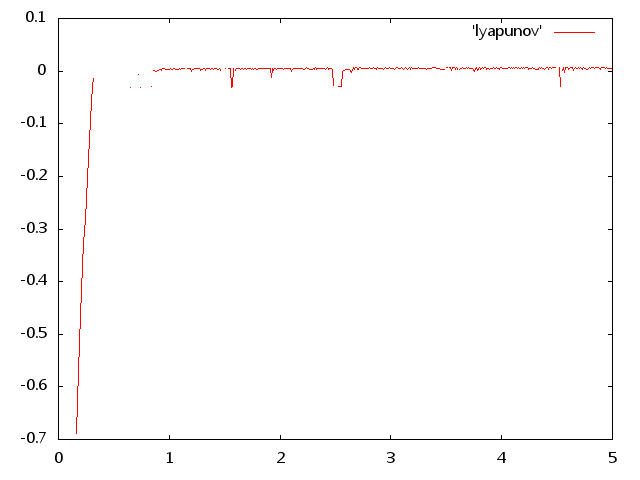
\includegraphics[width=4in]{lyapunov.png}
\end{center}

下面是 Logistic 映射对应的两个图. 可以看到和书上是一致的. 这表明我们的代码是正确的.
\begin{center}
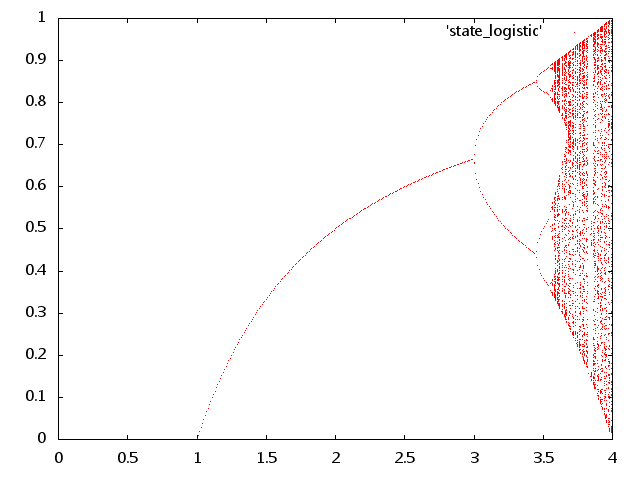
\includegraphics[width=4in]{state_logistic.png}
\end{center}

\begin{center}
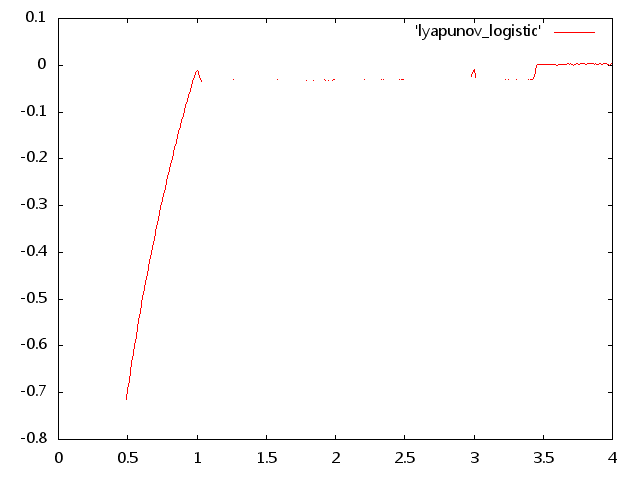
\includegraphics[width=4in]{lyapunov_logistic.png}
\end{center}

\end{document}